\subsection{Glyph: \glyph{Empty Set}}
\label{sec:emptySet}

It is useful to have the ability to represent the creation of an entity or a state from an unspecified source, that is, from something that one does not need or wish to make precise.  For instance, in a model where the production of a protein is represented, it may not be desirable to represent all of the amino acids, sugars and other metabolites used, or the energy involved in the protein's creation.
Similarly, we may not wish to bother representing the details of the destruction or decomposition of some biochemical species into a large number of more primitive entities, preferring instead to simply say that the species ``disappears into a sink''.
Yet another example is that one may need to represent an input (respectively, output) into (respectively, from) a compartment without explicitly representing a transport process from a source (respectively, to a target).

For these and other situations, SBGN defines a single glyph representing the involvement of an external pool of entities.
The symbol used in SBGN is borrowed from the mathematical symbol for ``empty set'', but it is important to note that it does not actually represent a true absence of everything or a physical void---it represents the absence of the corresponding structures in the model, that is, the fact that the external pool is conceptually outside the scope of the map.

A frequently asked question is, why bother having an explicit symbol at all?
The reason is that one cannot simply use an arc that does not terminate on a node, because the dangling end could be mistaken to be pointing to another node in the map.  This is specially true if the map is rescaled, causing the spacing of elements in the map to change.
The availability and use of an explicit symbol for sources and sinks is crucial.

\begin{glyphDescription}

\glyphSboTerm
SBO:0000291 ! empty set


\glyphIncoming
Zero or one \glyph{production} arcs (\sect{production}).



\glyphOutgoing
Zero or one \glyph{consumption} arcs (\sect{consumption}).


\glyphContainer
An \glyph{empty set} is represented by a circular shape crossed by a bar linking the lower-left and upper-right corners of the circle's bounding box, as shown in \fig{emptySet}.

\glyphLabel
None.

\glyphAux
None.

\end{glyphDescription}

\begin{figure}[H]
  \centering
  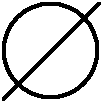
\includegraphics{images/emptySet}
  \caption{The \PD glyph for \glyph{empty set}.}
  \label{fig:emptySet}
\end{figure}

% The following is for [X]Emacs users.    Please leave in place.
% Local Variables:
% TeX-master: "../sbgn_PD-level1"
% End:
